\documentclass[a4paper,english,10pt]{article}

\usepackage[applemac]{inputenc}		% french special caracters (�, �, �, ...)
\usepackage[pdftex]{graphicx}				% to include figure in the document
\usepackage[footnotesize]{caption}      	% caption of table and figure in footnote size
\usepackage{color}                     			% texte en couleurs
\usepackage{subfig}					% allow the use of subfigure in the figure environment
\usepackage{fancyhdr}				% change header and footer
\usepackage{hyperref} 				% make hyperref in the pdf document
\usepackage{geometry}  				% change de geometry of the page
%\usepackage{eurosym}				% use of euro symbol
%\usepackage{floatflt}   				% for floating figure
\usepackage{multicol}    			% multicolumn document
\usepackage{multirow}    			% multicolumn document
\usepackage[Glenn]{fncychap}            	% formatage des titres de chapitres
%\usepackage{fancyvrb}                   		% pour afficher du code
%\usepackage{amsmath}				% math package
%\usepackage{sidecap}				% caption at le left or right side of the figures
%\usepackage{lettrine} 				% emploi de lettrine au debut du chapitre
\usepackage{fancyvrb}

\geometry{a4paper,tmargin=3cm,bmargin=2.5cm,lmargin=4cm,rmargin=3cm}
\pagestyle{headings}
\fancyfoot[C]{  \thepage \ }
\bibliographystyle{apalike}



%==========================pour les images================================
\graphicspath{{images/graphes/},{images/diagrammes/},
{images/illustrations/}, {images/}}
\DeclareGraphicsExtensions{.jpg,.png, .tiff, .pdf}

%==========================num�rotations==================================
\setcounter{tocdepth}{3}                % affiche jusqu'aux susubsections dans toc
\setcounter{secnumdepth}{3}             % chapitres et sections numrots
\setlength{\tolerance}{1000}             % tolrance pour l'espace entre les mots

%==========================pour les couleurs===============================
\definecolor{coolSection}{RGB}{223,0,0}
\definecolor{coolSubSection}{rgb}{0.2,0,0.5}
\definecolor{coolGreen}{RGB}{22,109,15}
\definecolor{red}{RGB}{255,0,0}


%=======================en-t�te et pieds de page==================================

\pagestyle{fancy}
\fancyhf{}
\fancyhead[L]{\leftmark}
\fancyfoot[R]{\thepage}

%==================== DOCUMENT =================================


\begin{document}

\title{
\begin{figure}[!h]

\includegraphics[width=\linewidth]{SmartRoot_logo}
\end{figure}
{\Huge Quick Start Guide}\\ \vspace{10mm}
 How to install, setup and use SmartRoot
 }
\normalsize

\maketitle

\setcounter{tocdepth}{1}   
\tableofcontents
\vspace{10pt}
\rule{0.9\linewidth}{1pt}
\vspace{10pt}

This small document presents briefly how to install, setup and use SmartRoot. \\

For more detailed informations about SmartRoot, you might want to read either the User Guide\footnote{\url{www.uclouvain.be/en-smartroot}} or the related paper:\\

\noindent \fbox{\parbox{\linewidth}{ \href{http://www.plantphysiol.org/content/early/2011/07/19/pp.111.179895.abstract}{Guillaume Lobet, Lo�c Pag�s and Xavier Draye. \textbf{A Novel Image Analysis Toolbox Enabling Quantitative Analysis of Root System Architecture.} 2011 Plant Physiology 157 doi:10.1104/pp.111.179895}}}

\newpage


{\color{coolSection}\section{First steps}}

{\color{coolSubSection}\subsection{System requirement}}

\begin{description}
\item [Memory:] At least 1024 MB of RAM for a good functioning
\item [Java:] SmartRoot works with Java 1.5 or higher
\item [Database (optional):] SmartRoot can export data to .csv text files but also directly into a database. For Windows we present how to setup a MS Access database connection. For Mac OS X and Linux (Ubuntu), we present how to setup a MySQL connection. People who does not have MS Access on Windows can follows similar steps as for Linux and Mac OS to install a MySQL database.
\end{description}

%%%%%%%%%%%%%%%%%%%%%%

{\color{coolSubSection}\subsection{Installation files}}

\noindent Inside the SmartRootSetup.zip file, you will find the following folders and files:\\

\begin{description}
\item [SmartRoot Quick Start.pdf] This document. Helps you to quickly install SmartRoot.
\item[SmartRoot User Guide.pdf] Complete user guide to learn all the SmartRoot functionalities. 
\item [Quick Start Images folder] Four images to learn how to trace root with SmartRoot. Instructions are written directly on the images.
\item [SmartRoot folder] The SmartRoot program in itself. Contains four .jar files: Smart\_Root.jar, Image\_Explorer.jar, jcommon-1.0.16.jar, jfreechart-1.0.13.jar and mysql-connector-java-5.1.7-bin.jar. This is the folder you will have to copy in the ImageJ folder (see below).
\end{description}

%%%%%%%%%%%%%%%%%%%%%%

\newpage
{\color{coolSection}\section{Windows installation}}

\begin{enumerate}
\item Configure the database (optional)
\item Install ImageJ and SmartRoot
\item Use the Quick start images
\end{enumerate}

%{\color{coolSubSection}\subsection{Java 1.5 installation}}
%
%Download Java 1.5 from the following page (choose the Java Runtime Environment (JRE) 5.0 Update 22) and install it.\\
%
%\noindent \fbox{\parbox{\linewidth}{\url{http://java.sun.com/javase/downloads/index_jdk5.jsp}}}\\ 

{\color{coolSubSection}\subsection{Database installation and connection}}
\label{dbwin}

\noindent To configure an ODBC data source that connects SmartRoot to a MS Access database:\\

\begin{enumerate}
\item Close the ImageJ program if it is running
\item Starts the \verb|ODBC administrator| from the \\ \verb|Control panel > Administrative tools > ODBC administrator|
\item Under the tab \verb|User DSN|, click \verb|Add…|
\item A list of database drivers is displayed. Select \verb|Microsoft Access Driver|, and click \verb|Finish|. You may need to contact your DB vendor if the driver is not in that list.
\item In the next dialog box, specify \verb|SmartRoot| in the \textbf{Data Source Name} field. In the \textbf{Database} area, click \verb|Create| to create a new database. Choose the directory in which you want to create the database, and name it \verb|SmartRoot.mdb| (in the upper left text field).
\item Click OK to validate and quit the ODBC administrator.\\
\end{enumerate}

When you launch SmartRoot (see below), the following message is displayed in the Results window of ImageJ if the connexion was successfully established:

\begin{Verbatim}[frame=single, commandchars=+\(\)]
SQL connection started on ODBC source SmartRoot
\end{Verbatim}

If the program failed to open the datasource, the message is:

\begin{Verbatim}[frame=single, commandchars=+\(\)]
The ODBC datasource 'SmartRoot' was not found.
You will not be able to write to a database.
\end{Verbatim}

{\color{coolSubSection}\subsection{SmartRoot installation\\}}

\begin{enumerate}
\item Download and install ImageJ 
\item Copy the SmartRoot folder in the \verb|Program Files > ImageJ > Plugins| folder.
\item Open ImageJ and choose \verb|Plugins > SmartRoot > SR Explorer|\\
\end{enumerate}

\noindent ImageJ download:\\

\noindent\fbox{\parbox{\linewidth}{\url{http://rsbweb.nih.gov/ij/download.html}\\
\footnotesize{If you do not have Java installed, please choose a version of ImageJ bundled with Java}}}\\\\

\noindent
\fbox{\parbox{\linewidth}{%
{\color{red}\textsc{Important:}}\\
If you are using {\color{coolSection} Windows 7}, all the components you are using together (in our case, Java, ImageJ and Access) have to be build on the same architecture (32bit or 64bit). \\
\noindent For instance,  if your Access software is 64bit, please choose the {\color{coolSubSection}ImageJ bundled with 64 bit Java} in the ImageJ download page. 
}}\\

%%%%%%%%%%%%%%%%%%%%%%%%%%%%%

\newpage

{\color{coolSection}\section{Mac OSX installation}}

\begin{enumerate}
\item Install and configure MySQL database (optional)
\item Install ImageJ and SmartRoot
\item Use the Quick start images
\end{enumerate}

{\color{coolSubSection}\subsection{MySQL installation and configuration}}
\label{dbmac}

\subsubsection{Installation}
Download the latest MySQL version from:\\ 

\noindent \fbox{\parbox{\linewidth}{\url{http://dev.mysql.com/downloads/}}}\\

\noindent
Open the disk image then install MySQL by double clicking on the \verb|mysql-...-.pkg| icon. \\
Also install the \verb|MySQLStratupItem.pkg| and \verb|MySQL.prefPane|.\\

\noindent
Open the \verb|System Preferences>MySQL| and start the MySQL server.

\subsubsection{Configuration}

Download the MySQLWorkbench from the following link and install it \\

\noindent \fbox{\parbox{\linewidth}{\url{http://dev.mysql.com/downloads/workbench}}}\\

\noindent 
Open the application and click \verb|New Connection|. Fill the fields as follow:\\

\noindent
\fbox{ \parbox{\linewidth}{%
\textbf{Connection Name:} choose the name you want (ex: SmartRoot) \\ 
\textbf{Connection Method:} Standart (TCP/IP)\\
\textbf{Hostname:} localhost \\ 
\textbf{Port:} 3306 \\ 
\textbf{Username:} choose the name you want (ex: root) \\ 
\textbf{Password:} leave it empty \\ 
\textbf{Default Schema:} leave it empty }} \\

\noindent
Open the connection and create a new schema called \verb|SmartRoot| by clicking the '+' sign.\\
Name the new schema SmartRoot and create it. \\
Click the \verb|Refresh| button to see your newly created database.


{\color{coolSubSection}\subsection{SmartRoot installation \\}}

\begin{enumerate}
\item Download and install ImageJ 
\item Copy the SmartRoot folder in the \verb|Applications > ImageJ > Plugins| folder.
\item Open ImageJ and choose \verb|Plugins > SmartRoot > SR Explorer|\\
\end{enumerate}

\noindent ImageJ download:\\

\noindent\fbox{\parbox{\linewidth}{\url{http://rsbweb.nih.gov/ij/download.html}}}

\newpage
{\color{coolSubSection}\subsection{Connect SmartRoot to the database}}

Once you have installed SmartRoot, open it.
The following message is displayed in the Results window of ImageJ if the connexion was successfully established:\\

\begin{Verbatim}[frame=single, commandchars=+\(\)]
SQL connection started 
\end{Verbatim}

\noindent If the program failed to open the datasource, the message is:

\begin{Verbatim}[frame=single, commandchars=+\(\)]
The specified datasource was not found.
You will not be able to write to a database.
\end{Verbatim}

\noindent
If you see this error message, go in the SmartRoot window, choose the \verb|Settings| tab and find the \verb|SQL options| panel. Fill the fields as follow:\\

\noindent
\fbox{\parbox{\linewidth}{%
\textbf{Driver class name:} com.mysql.jdbc.Driver\\
\textbf{Connection URL:} jdbc:mysql://localhost/SmartRoot\\
\textbf{Connection user name:} the username you choose previously\\
\textbf{Connection password:} leave empty }}\\
	
\noindent Press the \verb|Save Prefs| then \verb|Restart server| button. You should see the correct message saying the connection started


%%%%%%%%%%%%%%%%%%%%%%%%%%%%%%%%%%%%
\newpage
{\color{coolSection}\section[Linux installation]{Linux installation (Ubuntu distribution)}}

\begin{enumerate}
\item Install MySQL (optional)
\item Install ImageJ
\item Install ImageJ and SmartRoot
\item Configuring the database (optional)
\item Use the Quick start images
\end{enumerate}

%{\color{coolSubSection}\subsection{Java 1.5 installation}}
%
%In the terminal window type:\\
%
%\begin{Verbatim}[frame=single, commandchars=+\(\)]
%$sudo apt-get install sun-java5-jre
%\end{Verbatim}


{\color{coolSubSection}\subsection{MySQL installation and configuration}}
\label{dblin}

\subsubsection{Installation}

In the terminal window type:\\

\begin{Verbatim}[frame=single, commandchars=+\(\)]
$sudo apt-get install mysql-server
$sudo apt-get install mysql-query-browser
\end{Verbatim}

\noindent
While installing, you will be asked to setup username and password for your database connection. Leave the default values.

\subsubsection{Configuration}

Open MySQL Administrator. To connect to the database fill the form as follow:\\

\noindent
\fbox{\parbox{\linewidth}{%
\textbf{Server Hostname:} localhost\\
\textbf{Username:} root\\
\textbf{Password:} Leave empty}}\\

\noindent
In the MySQL Administrator window, choose \verb|Catalog| in the left panel. 

\noindent
In the bottom left panel \verb|Schemata|, right-click and choose \verb|Create Schema|. \\
Name it \verb|SmartRoot|



{\color{coolSubSection}\subsection{ImageJ installation}}

\noindent
In the terminal window type:\\

\begin{Verbatim}[frame=single, commandchars=+\(\)]
$sudo apt-get install imagej
\end{Verbatim}



{\color{coolSubSection}\subsection{SmartRoot installation}}

Copy the \verb|SmartRoot| folder from the \verb|SmartRootSetup| folder you downloaded into the \verb|usr/share/imagej/plugins/| folder\\

\noindent
In the terminal window type:\\

\begin{footnotesize}
\begin{Verbatim}[frame=single, commandchars=+\(\)]
$sudo mv /home/(+color(red)where_you_unzipped)/SmartRootPlug/SmartRoot /usr/share/imagej/plugins
\end{Verbatim}
\end{footnotesize}

\noindent To launch SmartRoot open ImageJ and choose \verb|Plugins > SmartRoot > SR Explorer|\\

\noindent
\fbox{\parbox{\linewidth}{%
{\color{red}\textsc{Important:}}\\
Ubuntu use the {\color{coolSubSection}Alt-key} to grab and move windows. SmartRoot use the same key to automatically trace roots. In order to use SmartRoot correctly, you have to change one Ubuntu parameter:\\

\noindent Go to System $>$ Preferences $>$ Windows and set the Movement key to Super.}}\\


{\color{coolSubSection}\subsection{Connect SmartRoot to the database}}

Once SmartRoot is installed, open it.

\noindent
The following message is displayed in the Results window of ImageJ if the connexion was successfully established:\\

\begin{Verbatim}[frame=single, commandchars=+\(\)]
SQL connection started 
\end{Verbatim}

\noindent If the program failed to open the datasource, the message is:

\begin{Verbatim}[frame=single, commandchars=+\(\)]
The specified datasource was not found.
You will not be able to write to a database.
\end{Verbatim}

\noindent
If you see this error message, go in the SmartRoot window, choose the \verb|Settings| tab and find the \verb|SQL options| panel. Fill the fields as follow:\\

\noindent
\fbox{\parbox{\linewidth}{%
\textbf{Driver class name:} com.mysql.jdbc.Driver\\
\textbf{Connection URL:} jdbc:mysql://localhost/SmartRoot\\
\textbf{Connection user name:} the username you choose previously (default = root)\\
\textbf{Connection password:} leave empty }}\\
	
\noindent
Press the \verb|Save Prefs| then \verb|Restart server| button. You should see the correct message saying the connection started

%%%%%%%%%%%%%%%%%%%%%%%%%%%%%%%%%%%%%%%%%






\label{install}

\newpage

{\color{coolSection}\section{Quick Start SmartRoot}}

In order to learn how to use SmartRoot, open the different tutorial images inside the software (start with the image quick\_start\_1.tif). To open an image in Smart root, just find it on your computer in the Explorer window (fig. \ref{sr_win}). Follow the instruction on the image to learn how to trace roots.\\

\begin{figure}[htbp]
\begin{center}
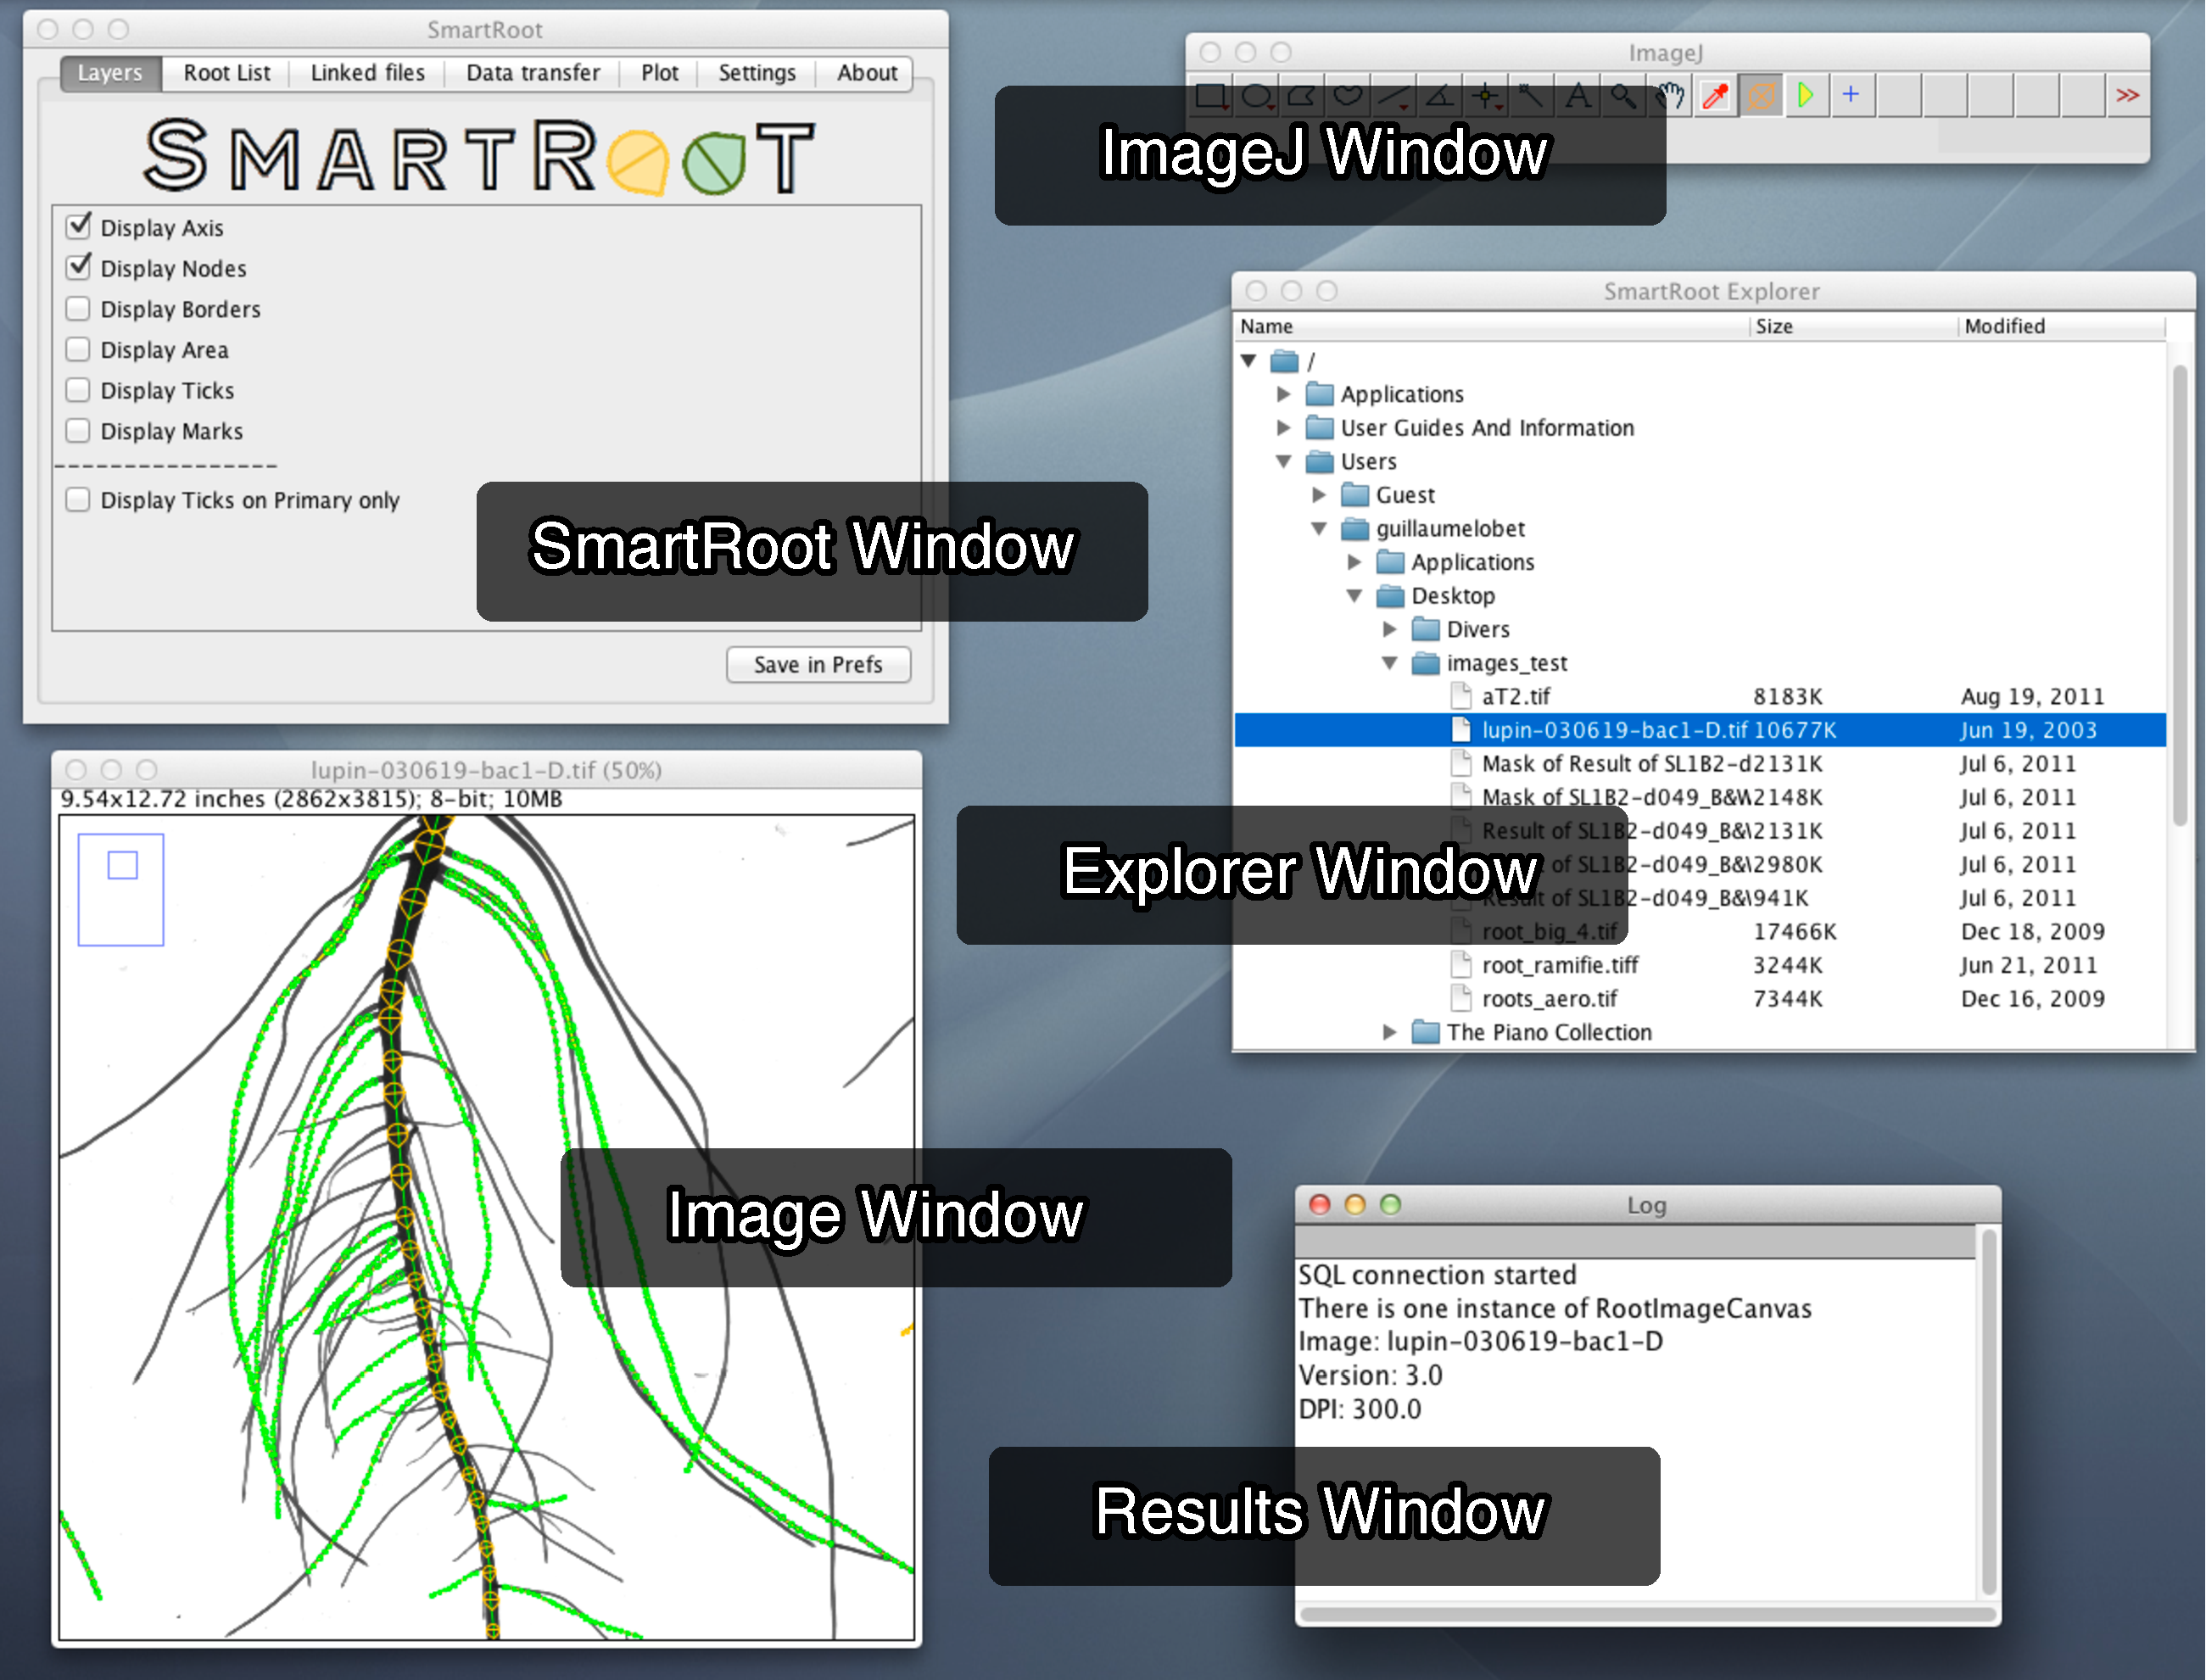
\includegraphics[width=\linewidth]{SR_windows_1}
\caption[]{\textbf{SmartRoot different windows}}
\label{sr_win}
\end{center}
\end{figure}


%%%%%%%%%%%%%%
\newpage
%{\color{coolSection}\section{How to trace a root?}}
{\color{coolSection}\section{Tracing roots}}

\begin{flushright}
{\color{coolSection}\textsc{{\Large Manual tracing}}}
\end{flushright}
\noindent \fbox{\parbox{\linewidth}{ 
\begin{enumerate}
\item Select the {\color{red}Trace} tool
\item Check {\color{red}Display nodes} and {\color{red}Display axis} in the Layer tab
\item {\color{red}Click} inside a root to place a node. 
\item Keep going until the end of the root
\item {\color{red}Double click} to end the root
\item Choose a name for the newly created root
\end{enumerate}}}\\
\vspace{20pt}
%
\begin{flushright}
{\color{coolSection}\textsc{{\Large Semi-automated tracing}}}
\end{flushright}
\noindent \fbox{\parbox{\linewidth}{ 
\begin{enumerate}
\item Select the {\color{red}Trace} tool
\item Check {\color{red}Display nodes} and {\color{red}Display axis} in the Layer tab
\item Maintain the {\color{red}Alt} key down
\item {\color{red}Click} inside a root to trace it. 
\item Choose a name for the newly created root
\end{enumerate}}}\\
\vspace{20pt}
%
%
%\newpage
%{\color{coolSection}\section{How to continue a root?}}

\begin{flushright}
{\color{coolSection}\textsc{{\Large Manually continuing a root}}}
\end{flushright}
\noindent \fbox{\parbox{\linewidth}{ 
\begin{enumerate}
\item Select the {\color{red}Trace} tool
\item Check {\color{red}Display nodes} and {\color{red}Display axis} in the Layer tab
\item {\color{red}Right click} on the first or last node of an existing root and choose {\color{red}Append node}. 
\item {\color{red}Click} inside the image to place a new node. 
\item Keep going until the end of the root
\item {\color{red}Double click} to end the root
\end{enumerate}}}
\vspace{20pt}
%
%
%
\newpage
\begin{flushright}
{\color{coolSection}\textsc{{\Large Automatically continuing a root}}}
\end{flushright}
\noindent \fbox{\parbox{\linewidth}{ 
\begin{enumerate}
\item Select the {\color{red}Trace} tool
\item Check {\color{red}Display nodes} and {\color{red}Display axis} in the Layer tab
\item Hold the {\color{red}Alt} key down
\item {\color{red}Click} on an existing node and {\color{red}drag} it a bit further. 
\end{enumerate}}}
\vspace{20pt}
%
%
%
%\newpage
%{\color{coolSection}\section{How to modify roots?}}

\begin{flushright}
{\color{coolSection}\textsc{{\Large Modifying nodes}}}
\end{flushright}
\noindent \fbox{\parbox{\linewidth}{ 
\vspace{10pt}
{\color{red}Right click} on an existing node. Choose on of the following action:
\begin{description}
\item[Append nodes:] Continue tracing in manual mode 
\item[Split root:] Split a root in two new roots.
\item[Remove node:] Remove the selected node.
\item[Remove all nodes (after):] Discard all node located distal to the selected node.
\item[Remove all nodes (before):] Discard all node located proximal to the selected node.\\
\end{description}}}
\vspace{20pt}
%
%
\begin{flushright}
{\color{coolSection}\textsc{{\Large Modifying roots}}}
\end{flushright}
\noindent \fbox{\parbox{\linewidth}{ 
\vspace{10pt}
{\color{red}Right click} inside an existing root. Choose on of the following action:
\begin{description}
\item[Bring to front:] Bring the selected root to the front of the list of roots. 
\item[Send to back:] Send the selected root to the back of the list of roots.
\item[Find laterals:] Check along the root axis for lateral roots creation. 
\item[Attach parent root:] Set a parent for the current root.
\item[Detach parent root:] Remove the relationship between a root and its parent.
\item[Detach children roots:] Remove the relationship between a root and all its children.
\item[Rename root:] Change the name of the selected root.
\item[Delete a root:] Remove the whole root.
\item[Reverse orientation:] Reverse the root orientation.
\item[Crop children:] Cut all roots whose first node is within the area of the selected root.
\end{description}}}\\
\vspace{20pt}

\newpage
\begin{flushright}
{\color{coolSection}\textsc{{\Large Connecting two existing roots}}}
\end{flushright}
\noindent \fbox{\parbox{\linewidth}{ 
\begin{enumerate}
\item Select the {\color{red}Trace} tool
\item Check {\color{red}Display nodes} and {\color{red}Display axis} in the Layer tab
\item {\color{red}Right click} on the first or last node of an existing root and choose {\color{red}Append node}. 
\item {\color{red}Right click} on the first or last node of an other existing root. 
\end{enumerate}}}
\vspace{20pt}

\begin{flushright}
{\color{coolSection}\textsc{{\Large Escaping the centering mechanism}}}
\end{flushright}
\noindent \fbox{\parbox{\linewidth}{ 
\begin{enumerate}
\item Select the {\color{red}Trace} tool
\item Check {\color{red}Display nodes} and {\color{red}Display axis} in the Layer tab
\item Hold the {\color{red}Control} key down and move a node for a {\color{coolSection}Diameter freeze}
\item Hold the {\color{red}Shift} key down and move a node for a {\color{coolSection}Align to border}
\item Combine {\color{red}Control}, {\color{red}Shift} and {\color{red}Alt} keys.
\end{enumerate}}}

%%%%%%%%%%%%%%%%%%%%%%%%

\newpage
{\color{coolSection}\section{SmartRoot window's tabs}}

\begin{flushright}
{\color{coolSection}\textsc{{\Large Layers tab}}}
\end{flushright}
\noindent \fbox{\parbox{\linewidth}{ 
\begin{center}
\begin{tabular}{lp{0.6\linewidth}}
\multirow{2}{*} {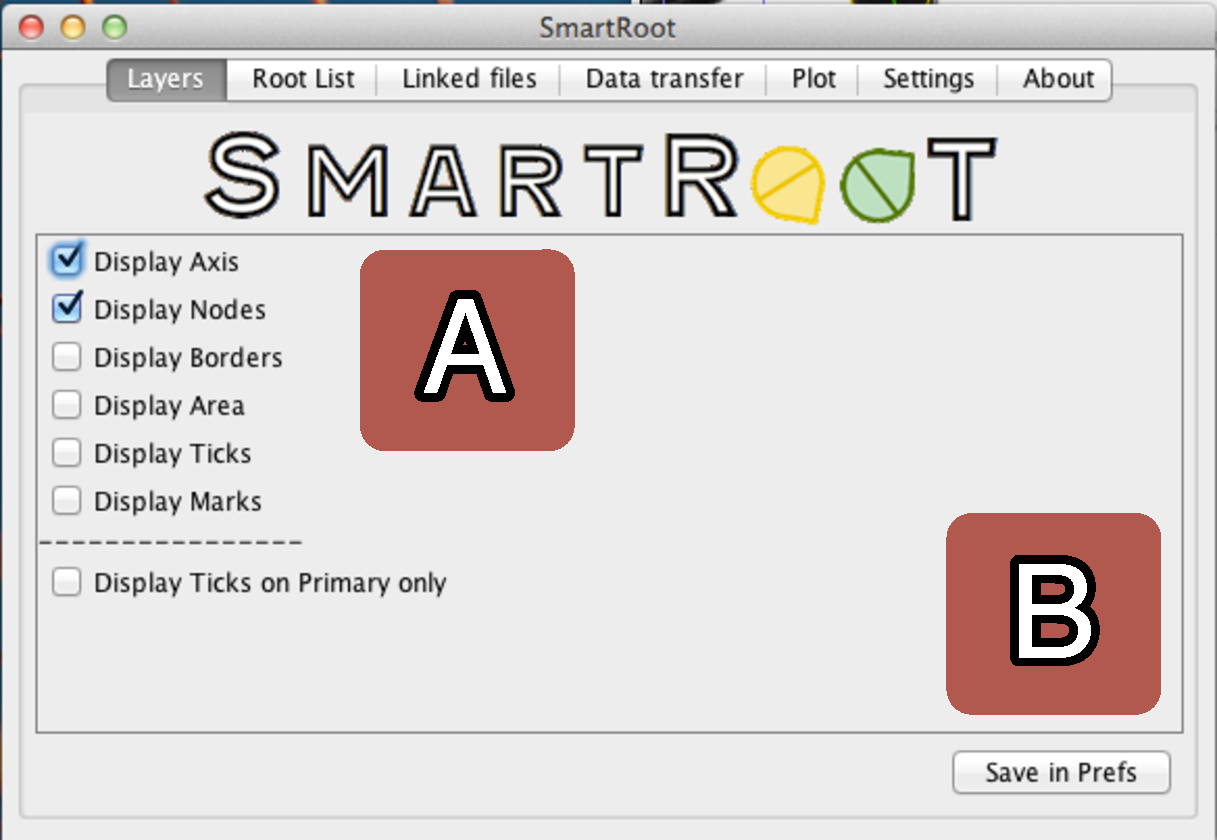
\includegraphics[width=0.3\linewidth]{layers}} & \textbf{A.} Type of layers.\\ 
 & \textbf{B.} Save your preferences.\\  \vspace{45pt}
\end{tabular}
\end{center}}}
\vspace{20pt}


\begin{flushright}
{\color{coolSection}\textsc{{\Large Root list tab}}}
\end{flushright}
\noindent \fbox{\parbox{\linewidth}{ 
\begin{center}
\begin{tabular}{lp{0.5\linewidth}}
\multirow{7}{*} {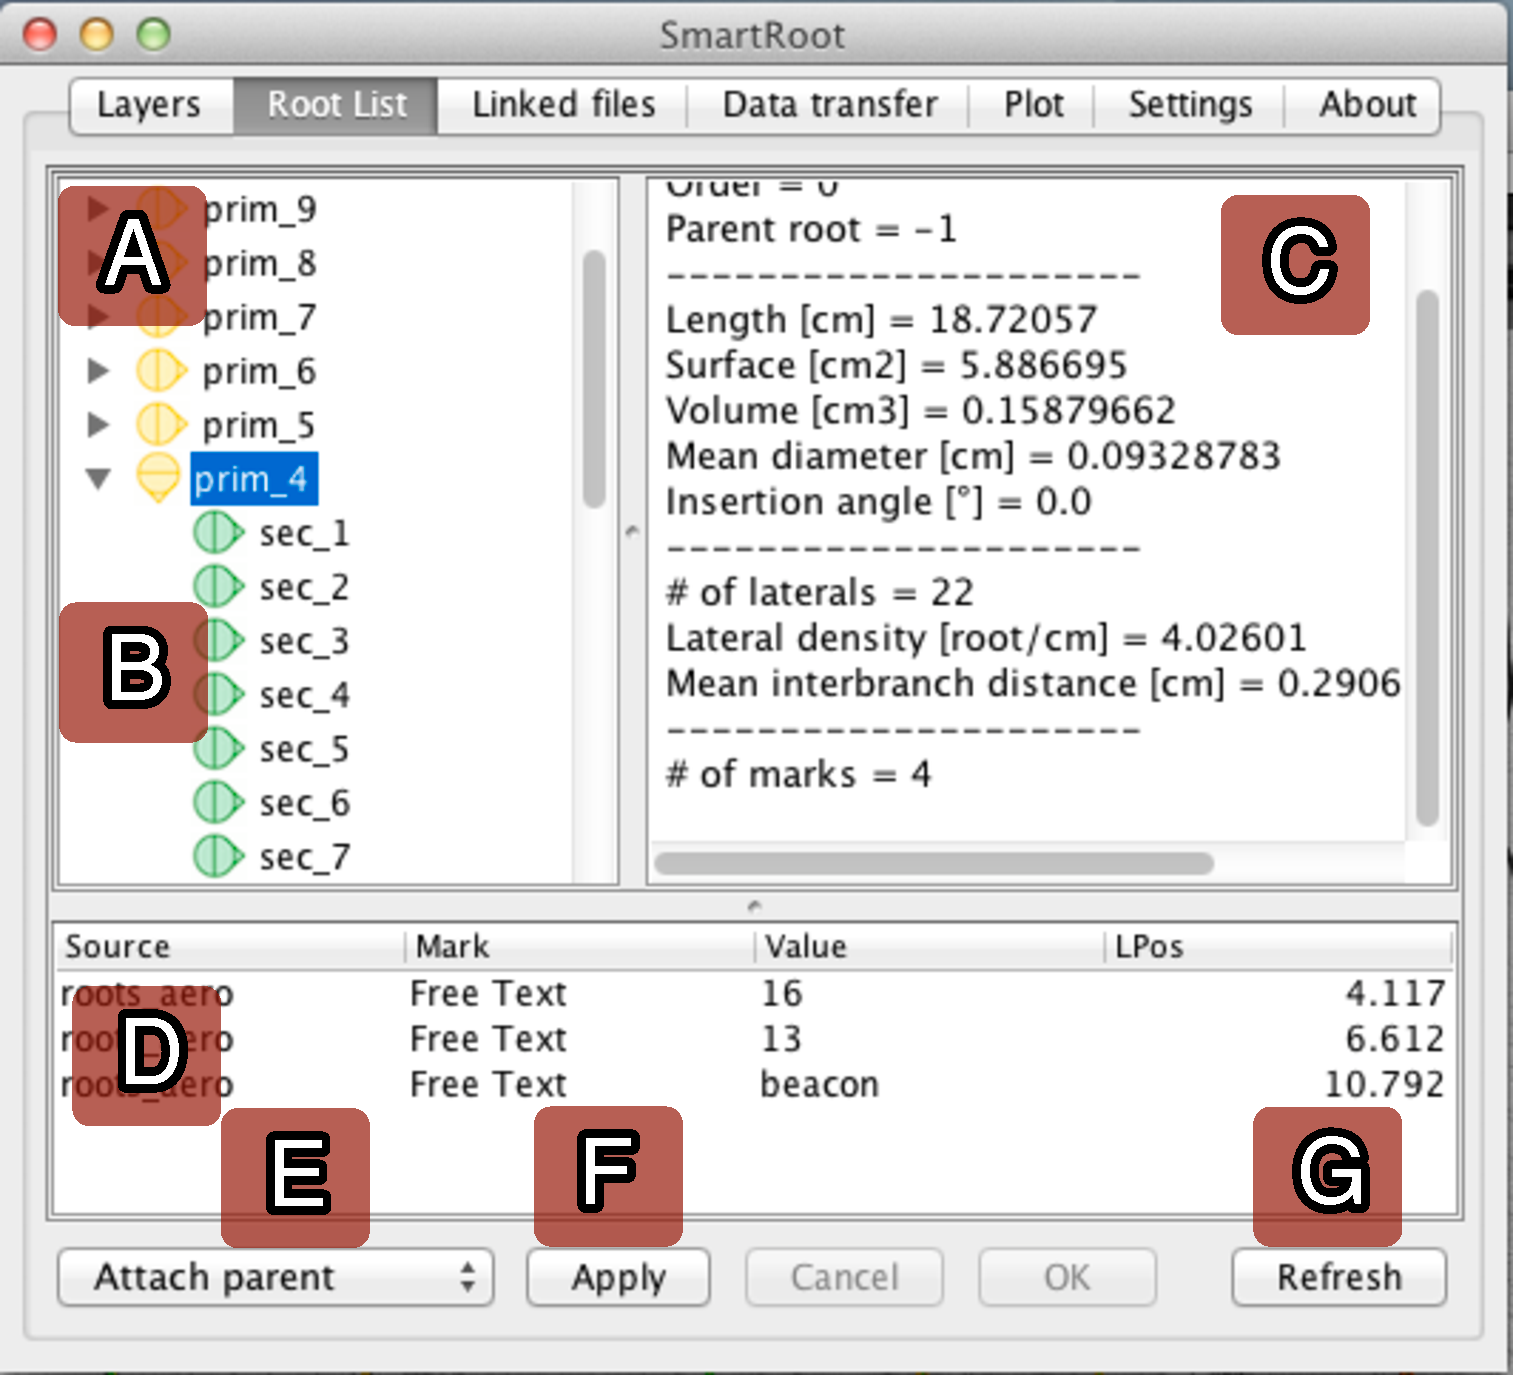
\includegraphics[width=0.4\linewidth]{root_list}} & \textbf{A.} Primary roots, in yellow.\\ 
 & \textbf{B.} Secondary roots, in green.\\ 
 & \textbf{C.} Informations about the selected root(s). \\ 
 & \textbf{D.} Marks of the selected root.\\ 
 & \textbf{E.} Perform actions on the selected root(s).\\
 & \textbf{F.} Validate the chosen action.\\ 
 &\textbf{G.} Refresh the root list \\
\end{tabular}
\end{center}
\begin{center}
\vspace{65pt}\rule{0.8\linewidth}{1pt}\vspace{15pt}
\begin{tabular}{p{0.1\linewidth}p{0.8\linewidth}}
\textbf{Actions:} & Delete root(s) | Delete mark(s) | Rename root\\
& Attach parent | Detach parent | Detach child(ren) | Find laterals
\end{tabular}
\end{center}}}
\vspace{20pt}

\begin{flushright}
{\color{coolSection}\textsc{{\Large Linked files tab}}}
\end{flushright}
\noindent \fbox{\parbox{\linewidth}{ 
\begin{center}
\begin{tabular}{lp{0.5\linewidth}}
\multirow{2}{*} {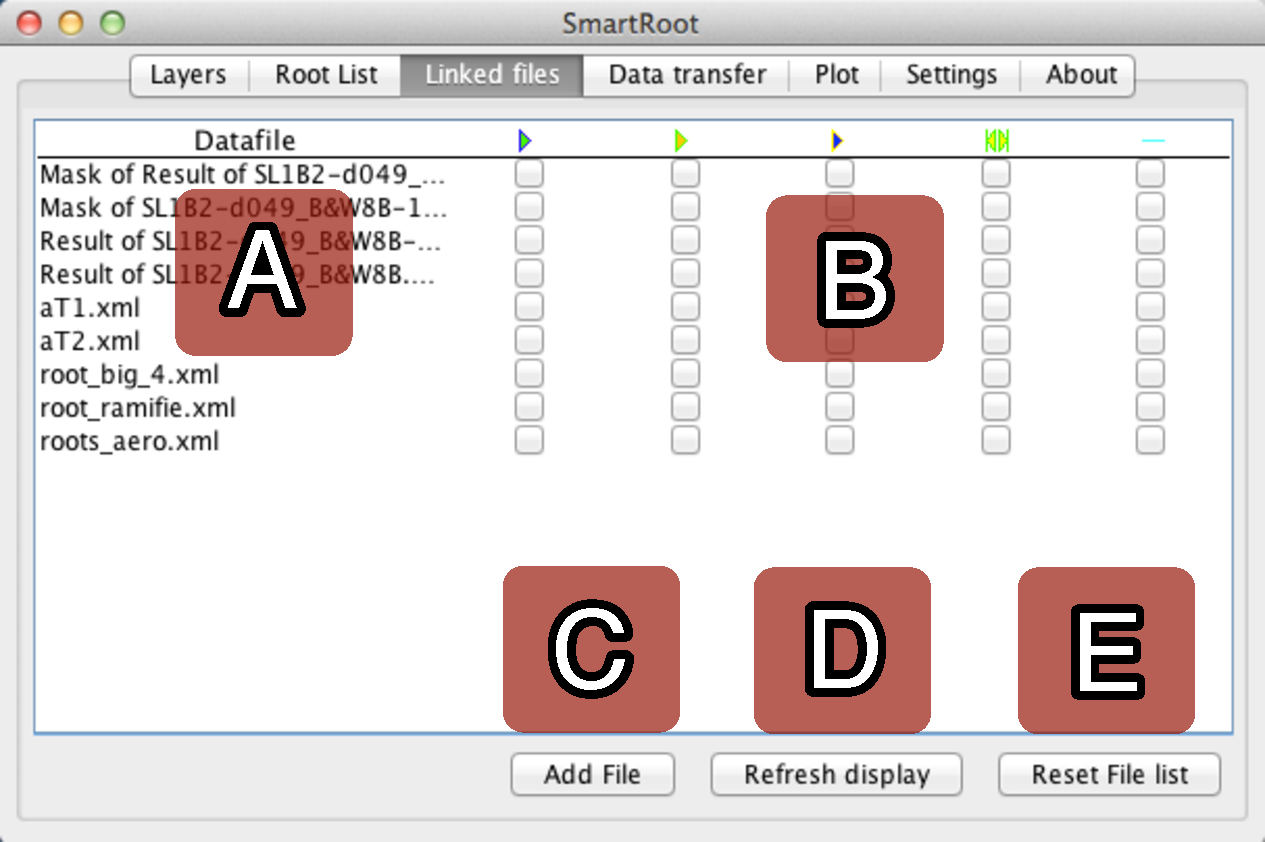
\includegraphics[width=0.4\linewidth]{linked_files}} & \textbf{A.} Files to link.\\ 
 & \textbf{B.} Marks to link.\\  
 & \textbf{C.} Add a file to the list.\\
 & \textbf{D.} Refresh the image display.\\
 & \textbf{E.} Refresh the list display.\\      \vspace{40pt}
\end{tabular}
\end{center}}}
\vspace{20pt}


\begin{flushright}
{\color{coolSection}\textsc{{\Large Data transfers tab}}}
\end{flushright}
\noindent \fbox{\parbox{\linewidth}{ 
\begin{center}
\begin{tabular}{lp{0.5\linewidth}}
\multirow{4}{*} {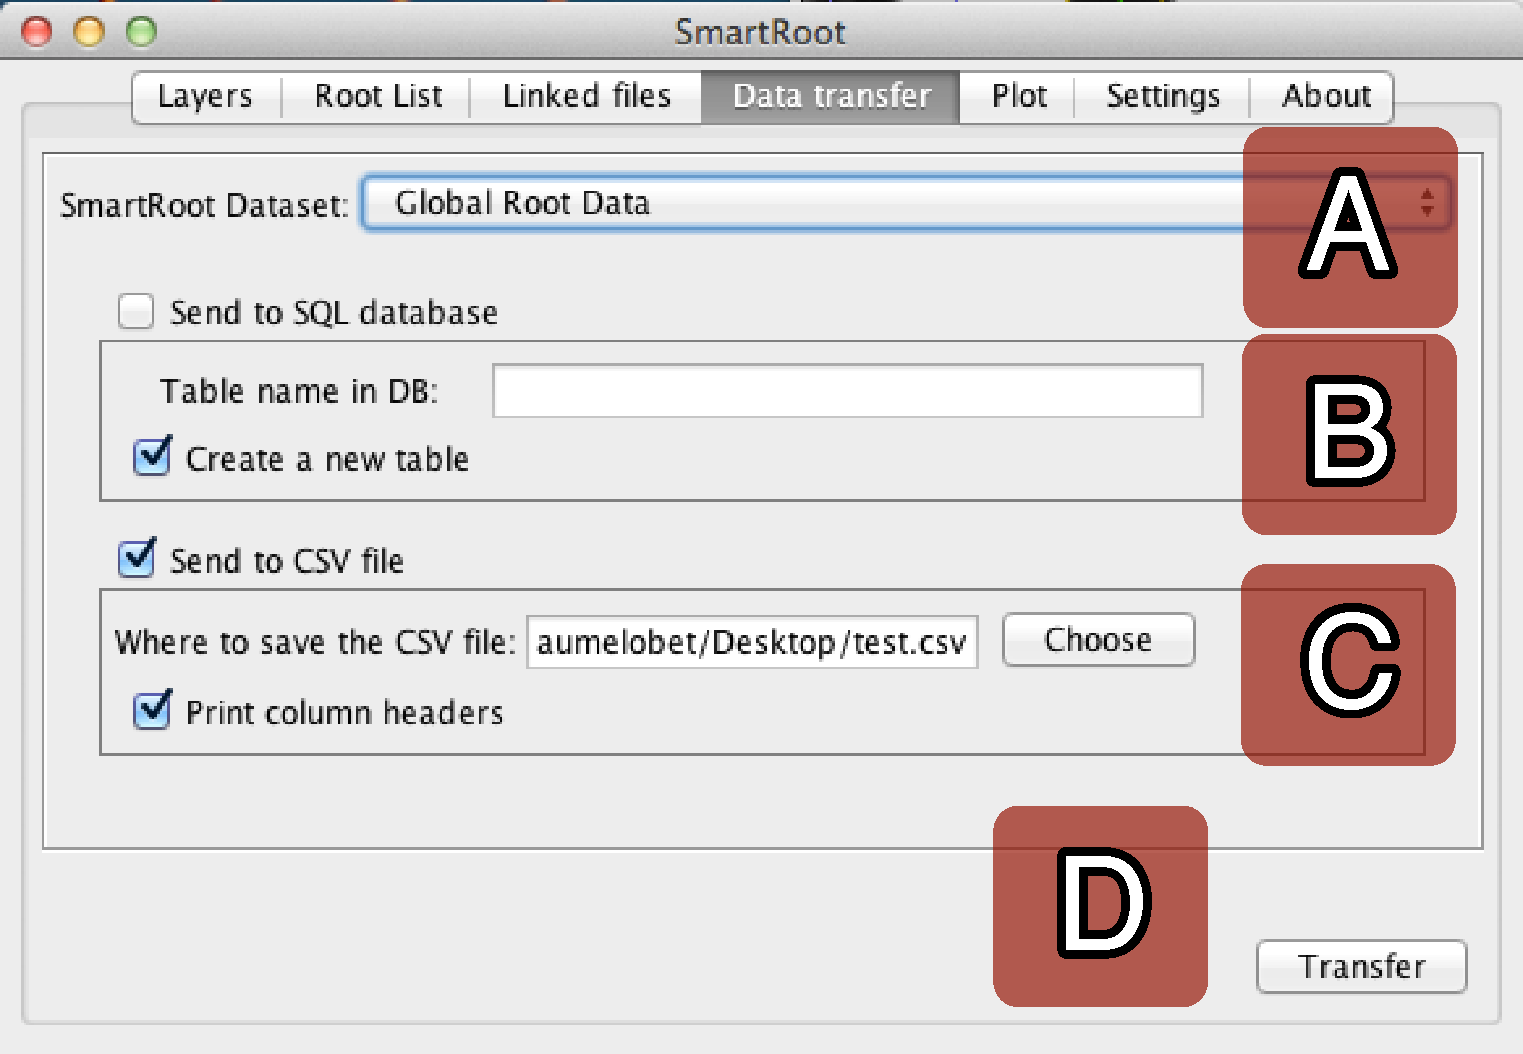
\includegraphics[width=0.4\linewidth]{data_transfers}} & \textbf{A.} List of SmartRoot datasets.\\ 
 & \textbf{B.} Export to SQL. \\ 
 & \textbf{C.} Export to CSV\\ 
 & \textbf{D.} Transfers button.\\ \vspace{40pt} 
\end{tabular}
\end{center}
\begin{center}
\vspace{20pt}\rule{0.8\linewidth}{1pt}\vspace{15pt}
\begin{tabular}{p{0.1\linewidth}p{0.8\linewidth}}
\textbf{Datasets:} & Global Root Data | All marks | Root Nodes | Root Length density\\
\end{tabular}
\end{center}}}
\vspace{20pt}

\begin{flushright}
{\color{coolSection}\textsc{{\Large Plot tab}}}
\end{flushright}
\noindent \fbox{\parbox{\linewidth}{ 
\begin{center}
\begin{tabular}{lp{0.6\linewidth}}
\multirow{5}{*} {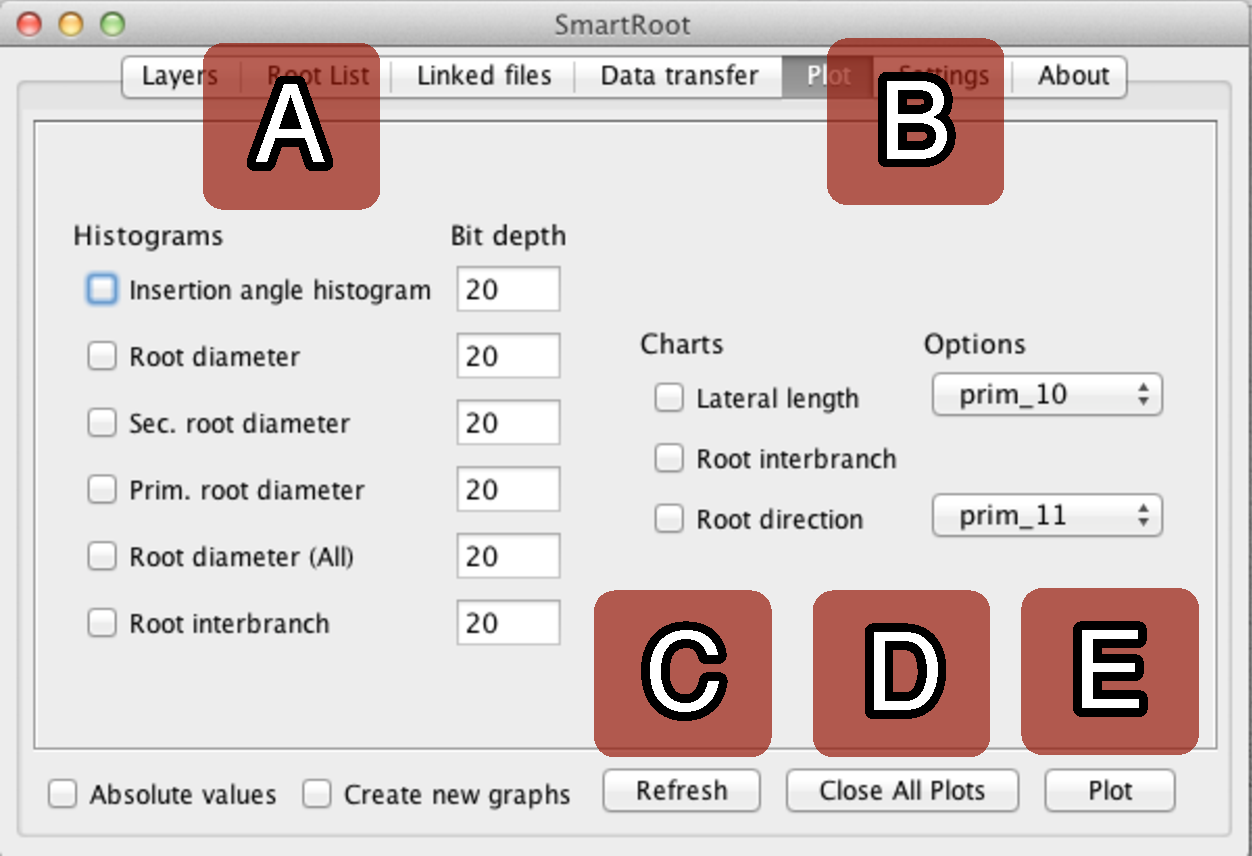
\includegraphics[width=0.4\linewidth]{SR_plot}} & \textbf{A.} Histograms.\\ 
 & \textbf{B.} Charts.\\ 
 & \textbf{C.} Refresh button. \\ 
 & \textbf{D.} Close all plots.\\ 
 & \textbf{E.} Plot the selected charts and histograms.\\ \vspace{35pt}
\end{tabular}
\end{center}}}
\vspace{20pt}


\begin{flushright}
{\color{coolSection}\textsc{{\Large Settings tab}}}
\end{flushright}
\noindent \fbox{\parbox{\linewidth}{ 
\begin{center}
\begin{tabular}{lp{0.6\linewidth}}
\multirow{5}{*} {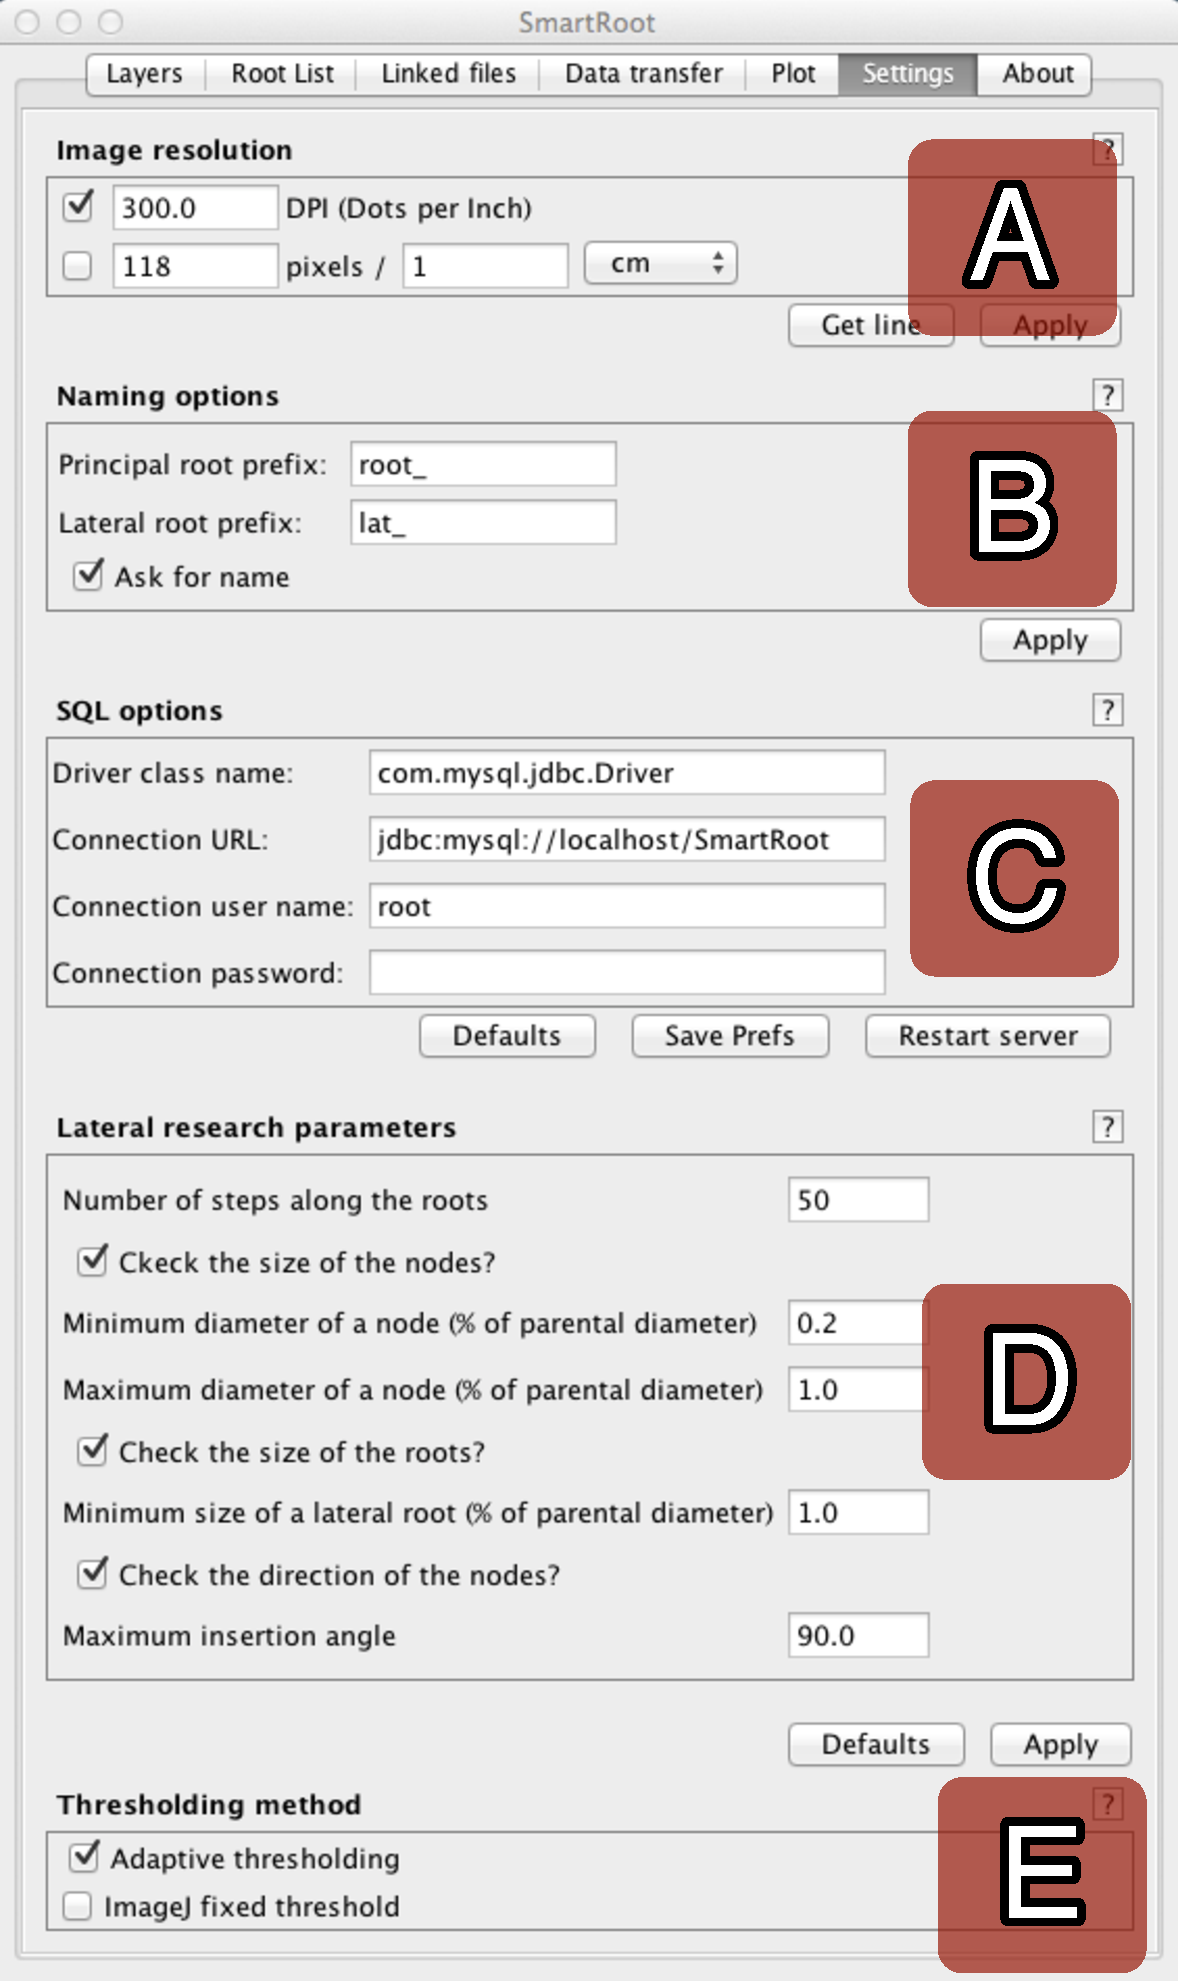
\includegraphics[width=0.2\linewidth]{settings}} & \textbf{A.} Image resolution.\\ 
 & \textbf{B.} Naming options.\\ 
 & \textbf{C.} SQL options. \\ 
& \textbf{D.} Lateral finding options. \\ 
 & \textbf{E.} Thresholding options. \\ \vspace{70pt}
\end{tabular}
\end{center}}}



\end{document}
